\section{Method/Approach}
\label{sec:method}

\subsection{Formal Definition}

We formally define a \emph{Material Evolution Knowledge Hypergraph} (\tool{}) as a directed labeled multi-hypergraph $\Hcal(M, E)$ \cite{ouvrardHypergraphsIntroductionReview2020}, where $M$ and $E$ denote a set of materials (also referred to as nodes) and the set of directed hyper-edges, respectively. 
Each (directed) hyper-edge $e=(e_s, e_t)\in E$ corresponds to a chemical or industrial \textit{process} $\mathbf{P_e}$, which transforms a set $e_s=\{m_1, \ldots m_p\}\subset M$ of inputs to a set $e_t=\{m_q, \ldots, m_r\}\subset M$ of outputs.
We refer to $e_s, e_t$ as the source and target of $e$, respectively.
% the process corresponding to $e$ transforms the source set $e_s =\{m_1, \ldots m_p\}$ of materials (the inputs of the process) to the target set $e_t=\{m_q, \ldots, m_r\}$ (the outputs of the process).
% the source $e_s$ is a \textit{process}, that uses as inputs a set of materials $m_1, \ldots m_p \in M$, and produces a set of outputs $m_q, \ldots, m_r \in M$.
%Each process requires a specific set of inputs, and produces a specific set of outputs. 
% \samarth{need to write in a more complete and formal manner}  
We use $\ell(e)=\mathbf{P}_e$ as the label for the hyperedge $e$.
There could be multiple processes $\mathbf{P}_{e_1}, \mathbf{P}_{e_k}$ transforming a source set $S$ to a target set $T$;
these would be represented as multiple hyper-edges $e_i=(S, T)$ with $\ell(e_i)=\mathbf{P}_{e_i}$.

We focus on the set $M$ of materials in the Harmonized System (which is a standardized numerical method of classifying traded products); all such materials have a valid Harmonized System (HS) Codes~\cite{hscode}.
We focus here on 6-digit HS codes, which represent aggregations of many products.

Our algorithm for producing ~\tool s is presented in Algorithm \ref{alg:tdn-pipeline}.
The ProcessGeneration method referred to in this Algorithm is a strategy that queries auxiliary resources $A$ to find processes, and filters the results based on several quality and relevance metrics. 

% OLD ALGORITH
\iffalse
\begin{algorithm}[h]
\caption{Bottom-Up Material Evolution Graph (System Process Overview) \samarth{rewrite using hypergraph terminology, expand lines 4,5,6}}
\label{alg:tdn-pipeline}
\begin{algorithmic}[1]

{\color{gray}
\REQUIRE number of iterations $n$, seed materials $s$, auxiliary data $A$, universe of allowable materials $\mathcal{M}$
\STATE $\text{Processes} \gets \emptyset$
\STATE $\text{Materials} \gets s$

\FOR{$i = 1, \ldots, n$}
    \STATE Update Processes from $\text{ProcessGeneration}(\text{Materials}, A)$
    \STATE Each process has a set of inputs, outputs $p_{in}, p_{out} \subset \mathcal{M}$
    \STATE Update Materials with $p_{in} \cup p_{out}$ for each new process
\ENDFOR
\RETURN $MEG = (\text{Materials}, \text{Processes})$ 
}
\end{algorithmic}
\end{algorithm}
\fi

% NEW ALGORITHM USING HYPEREDGE TERMS
\begin{algorithm}[h]
\caption{Bottom-Up \toolname (System Process Overview)} 
%\adscomment{Does this work/make sense as replacement?}
\label{alg:tdn-pipeline}
\begin{algorithmic}[1]
\REQUIRE number of iterations $n$, seed vertex set (seed materials) $s$, auxiliary hypergraph data $A$, universe of allowable vertices (materials) $\mathcal{V}$
\STATE $\text{Hyperedges (Processes)} \gets \emptyset$
\STATE $\text{Vertices (Materials)} \gets s$

\FOR{$i = 1, \ldots, n$}
    \STATE Update Hyperedges from $\text{ProcessGeneration}(\text{Vertices}, V)$
    \STATE Each hyperedge has a set of inputs, outputs e_{in}, e_{out} \subset \mathcal{V}$
    \STATE Update Vertices with $e_{in} \cup e_{out}$ for each new process
\ENDFOR
\RETURN $MEKH = (\text{Vertices}, \text{Hyperedges})$ 

\end{algorithmic}
\end{algorithm}

\subsection{Rationale}
The system architecture incorporates several design principles that address the requirements of industrial supply chain modeling. The directed hypergraph representation accommodates the multi-input, multi-output structure that characterizes industrial processes, providing a mathematical foundation that captures transformation complexity. The iterative pipeline methodology supports systematic network growth through discrete expansion cycles, maintaining traceability to source evidence and quality control through validation mechanisms at each stage. Integration with the Model Context Protocol enables LLM agents to access specialized tools and knowledge sources, thereby enhancing their reasoning capabilities and evidence retrieval processes while maintaining modularity. The command-line interface provides reproducible control over the pipeline workflow, supporting both research applications and operational supply chain analysis through user-directed network construction and inspection capabilities.

\subsection{Architectural Layers}
The bottom-up supply chain pipeline is built around a modular, iterative architecture designed to progressively construct a material evolution graph — a representation of how raw materials are transformed into intermediates for use in advanced products through industrial processes. The architecture consists of three interdependent layers that collectively support data representation, knowledge discovery, and user interaction.

\begin{figure}[htbp]
\centering
\begin{tikzpicture}[
    layer/.style={
        rectangle, rounded corners=3pt,
        minimum width=2.9in, minimum height=0.7in,
        text width=2.7in, align=center,
        font=\footnotesize, drop shadow
    },
    data/.style={layer, fill=blue!20, draw=blue!60, thick},
    orchestration/.style={layer, fill=green!20, draw=green!60, thick},
    interface/.style={layer, fill=orange!20, draw=orange!60, thick},
    component/.style={
        rectangle, rounded corners=2pt,
        minimum width=0.65in, minimum height=0.28in,
        text width=0.6in, align=center,
        font=\footnotesize, fill=white, draw=black!50, thick
    },
    arrow/.style={->, thick, draw=black!60},
    link/.style={thin, draw=gray!60}
]

% Layers (top to bottom)
\node[interface] (ui_layer) at (0,5.0) {
    {\begin{minipage}[t][0.5in][t]{2.6in}
      \centering
      \textbf{User Interaction Layer}\\
      CLI for seed materials, task monitoring, cache management
    \end{minipage}}
};

\node[orchestration] (orch_layer) at (0,2.9) {
    {\begin{minipage}[t][0.5in][t]{2.6in}
      \centering
      \textbf{Pipeline Orchestration Layer}\\
      LLM-driven task execution and validation via MCP
    \end{minipage}}
};

\node[data] (data_layer) at (0, 0.8) {
    {\begin{minipage}[t][0.5in][t]{2.6in}
      \centering
      \textbf{Data Representation Layer}\\
      Directed hypergraph with HS codes and metadata
    \end{minipage}}
};

% Components (kept clear of layer text)
\node[component] (cli)      at (-1.8,4.6) {CLI\\Interface};
\node[component] (monitor)  at (0,4.6)    {Task\\Monitor};
\node[component] (cache)    at (1.8,4.6)  {Cache\\Mgmt};

\node[component] (llm)       at (-2.7,2.5) {LLM\\Tasks};
\node[component] (mcp)       at (-0.9,2.5) {MCP};
\node[component] (manager)   at (0.9,2.5)  {Task\\Manager};
\node[component] (validator) at (2.7,2.5)  {Validator};

\node[component] (hypergraph) at (-2.7,0.4) {Directed\\Hypergraph};
\node[component] (meta)       at (-0.9,0.4) {Metadata\\Store};
\node[component] (hs)         at (0.9,0.4)  {HS\\Codes};
\node[component] (cache2)     at (2.7,0.4)  {Reference\\Cache};

% Inter-layer relations
\draw[<->, thick, draw=black!60] (ui_layer.south) -- (orch_layer.north);
\draw[<->, thick, draw=black!60] (orch_layer.south) -- (data_layer.north);

\end{tikzpicture}
\caption{Architectural Layers and Related Tools of the Bottom-Up Supply Chain Pipeline. %\samarth{Can we increase the font size
%in the white boxes?}
}
\end{figure}

\textbf{Data Representation Layer.}
The data representation layer defines the structure of the supply chain network as a directed hypergraph. This framework captures the complexity of industrial processes, including scenarios where several materials are inputs to a process and multiple outputs are possible. Additional metadata, such as harmonized system (HS) codes, process references, and a reference cache, are recorded to support semantic searches and detailed reasoning.

\textbf{Pipeline Orchestration Layer.}
The orchestration layer manages the execution of tasks that develop and refine the material evolution graph. These tasks—adding new materials, identifying process relationships, merging duplicate entries, and validating references—are assigned according to their function. Many are driven by large language models using resources and search tools configured through the Model Context Protocol.

\textbf{User Interaction Layer.}
Interaction with the pipeline is handled through a command-line interface. This interface allows users to provide seed materials, initiate or monitor expansion and validation tasks, maintain the reference cache, and review the current state of the evolving network. Each architectural layer operates independently; for example, the data layer can be updated with new sources without changes to orchestration or interface logic.

Each layer is designed for independent modification and extension; for instance, data sources can be updated without altering orchestration or interface logic.


\iffalse
\subsection{System Workflow}
The general workflow supports the automated discovery and interactive refinement of \toolname{}s, enabling control over both the scope of exploration and the level of detail achieved. The following sequence outlines the main steps involved in configuring and operating the \toolname{} construction pipeline. Many of the steps in the workflow are completed with the aid of one or more LLM agents. These agents are described in the System Pipeline and Agents section below.

\begin{enumerate}
\item The user sets up a research context using the command-line interface and specifies a primary seed material to begin network construction. Additional optional inputs may include specific intermediate material forms, reference documents for initial evidence, and a list of product families to guide downstream expansion.

\item If no optional configuration is provided, the pipeline begins with the seed material and incrementally identifies relevant materials and processes from that starting point.

\item The system performs a sequence of tasks: it expands the material set, identifies relevant industrial processes, collects and evaluates references, and removes unsupported connections in the network.

\item With each iteration, newly identified materials enable process mapping and downstream expansion. Material and process relationships are refined, with ongoing validation and traceability to supporting evidence.

\item The reference cache is updated as the workflow proceeds and indexed to support semantic search. Accumulated data and references from past iterations are used to inform subsequent expansions and validations.

\item The user may pause the workflow to review progress or modify parameters by adding materials or references, then resume network construction from the current state.

\end{enumerate}
\fi


\subsection {System Pipeline \& Agents}
The general workflow, as seen in figure \ref{fig:pipeline}, supports the automated discovery and interactive refinement of \toolname{}s, enabling control over both the scope of exploration and the level of detail achieved.
The implementation of the pipeline is organized into discrete, composable tasks, each responsible for a specific part of network expansion or refinement. These tasks can run independently or be combined into a complete iterative workflow. Many tasks rely on \textbf{task-specific LLM agents} that have access to structured auxiliary data and semantic search tools. There are currently 6 task-specific agents utilized in the pipeline: material classification agent, material finder agent, material manufacturing agent, process merging agent, reference reviewer agent, and url scorer agent.

\begin{figure}[h]
    \centering
    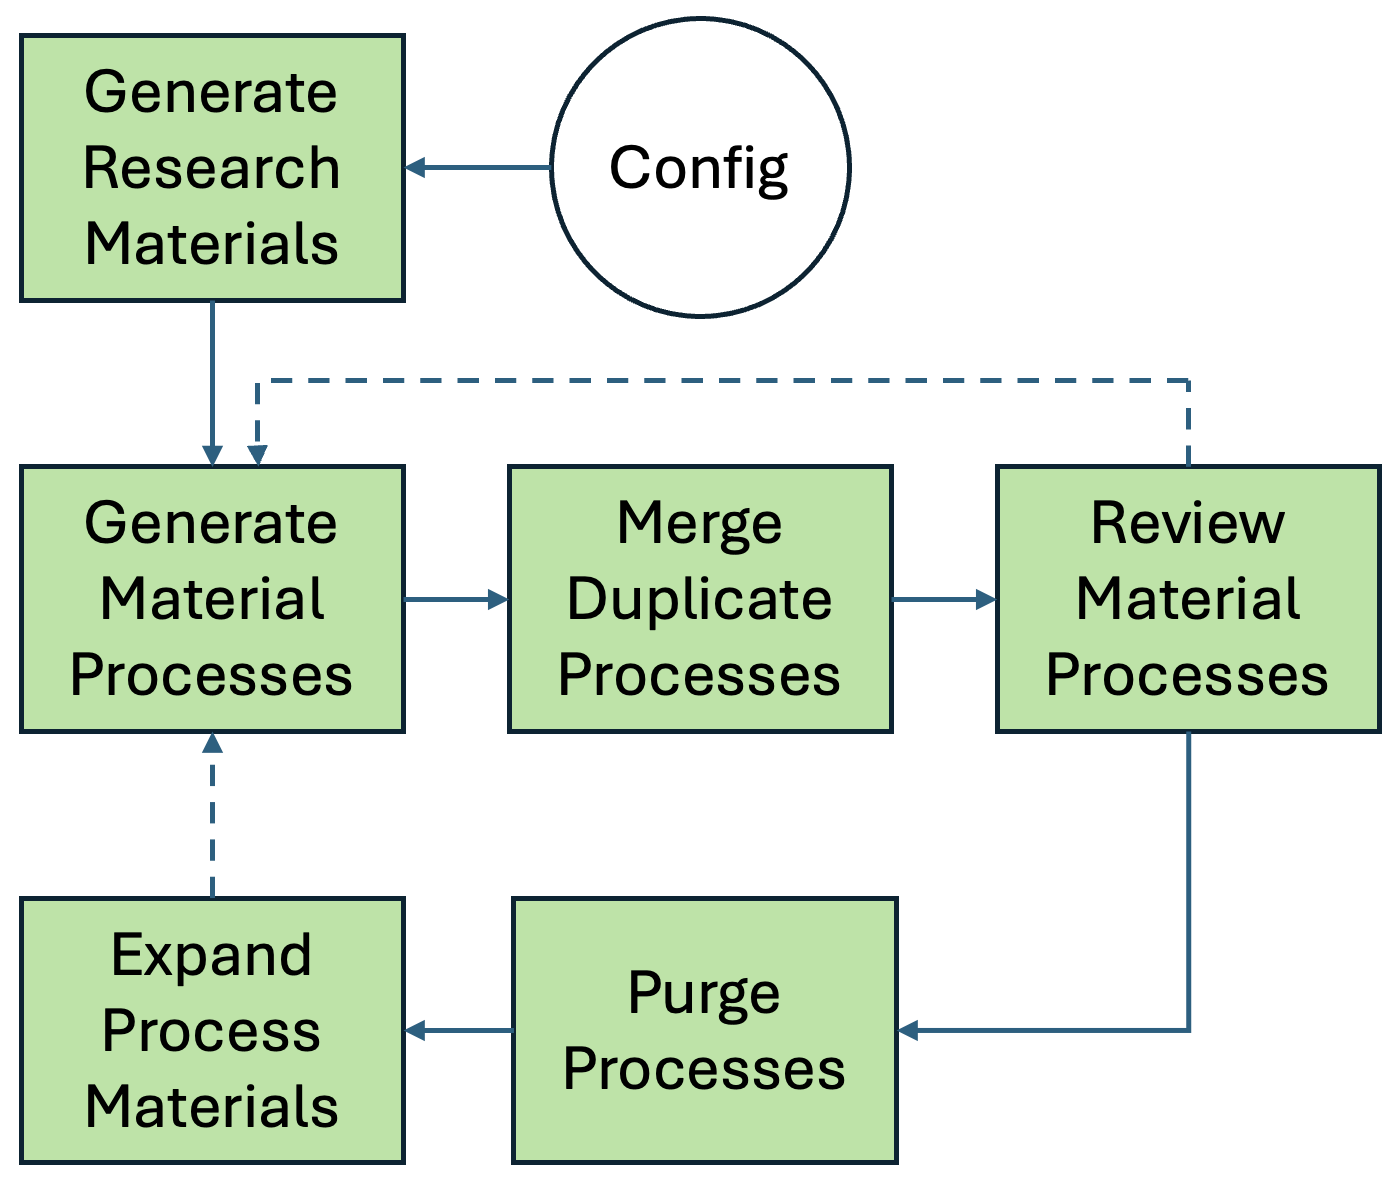
\includegraphics[width=0.9\linewidth]{images/pipeline-tasks2.png}
    \caption{Pipeline Tasks for the multi-agent system.  All tasks, with the exception of the Purge Processes task, use one or more LLM Agents to perform their tasks. }
    \label{fig:pipeline}
\end{figure}

%\subsubsection{System Process Overview: Bottom-Up Material Evolution Graph (MEG) Pipeline Algorithm}
%\mlwcomment{Why have a subsubsection here when it is the only subsubsection? Do we anticipate having more subsubsections, or would it be acceptable to just incorporate this into subsection 3.7?}
%\adscomment{Because the rest got moved to the Appendix. Good catch!}

\iffalse
The system process overview algorithm implements a bottom-up approach for constructing \toolname{} (\tool{}s) that map relationships between materials and manufacturing processes. The pipeline initializes a state object tracking materials, processes, and configuration parameters, with resumption capability from saved progress, then follows an iterative expansion strategy that first generates materials from seed inputs and enters a main loop, alternately discovering new manufacturing processes for existing materials and identifying additional upstream/downstream materials to support those processes. The algorithm employs a purging mechanism to remove processes lacking sufficient material support, ensuring realistic network dependencies. It continues to expand until reaching the maximum number of iterations or user termination, returning a directed hypergraph where the vertices represent the materials and the hyperedges represent the manufacturing processes that connect the input materials to the output products.
\fi

Lower-level algorithm breakdowns for Material Generation and Review, Process Generation and Merge, Review Processes, Purge Processes, and Upstream/Downstream Expansion are detailed in Appendix A.

\subsubsection{Material Generation}
Material generation initiates the pipeline, beginning with seed materials specified through the command-line interface. A \textbf{material classification agent} utilizes a large language model to analyze industrial contexts, chemical taxonomies, and harmonized trade nomenclatures, identifying materials that function as direct intermediates derived from existing nodes or downstream products positioned along the transformation chain. For each newly identified material, the agent extracts its canonical name, corresponding six-digit Harmonized System (HS) code, mined status indicating natural occurrence (ore, brine, mineral compound) versus refined/intermediate classification, aliases encompassing chemical synonyms and trade names, primary downstream applications, and formal HS description for standardized classification. This process operates iteratively, with each discovered material layer serving as input for subsequent generation rounds. Through multiple iterations, the method constructs a hierarchical node structure spanning naturally occurring forms, intermediate compounds, and advanced products.

\subsubsection{Process Generation and Merging}

Process generation constitutes the primary mechanism for network expansion beyond material nodes. A \textbf{manufacturing process agent} examines each material node to identify industrial transformations that either produce or consume the material. For processes that produce the material, the agent traces upstream manufacturing steps and input requirements. For processes that consume the material, the agent identifies downstream transformation pathways and resulting products. Each discovered process is recorded as a \textbf{hyperedge} containing a descriptive narrative of the transformation, scale designation (industrial, commercial, or laboratory), explicit lists of precursors and products linked by HS codes, and supporting references retrieved from web sources, technical reports, patents, and other documentation. The process generation task iterates across all material nodes to ensure comprehensive process discovery, with new processes introducing additional upstream or downstream materials that feed back into the material generation phase for continued network expansion.

Network growth produces multiple hyperedges that may describe identical processes with variations in descriptive language or reference sources. The process merging task addresses this redundancy by comparing all edges and identifying those with matching input and output material sets. When duplicate processes are detected, they are consolidated into a single canonical hyperedge that combines all supporting references from the original edges. This merging operation maintains network compactness and interpretability while preventing artificial inflation of the edge set through redundant process descriptions. A separate \textbf{reference review agent} evaluates the quality and reliability of supporting documentation later in the pipeline, ensuring the iterative approach between process generation and material generation drives systematic construction of the technology dependency network.

\subsection{Integration of External Tools and Data}

The system incorporates several external data sources and tools that are accessible to LLM agents during network construction. These components are integrated through the Model Context Protocol:

\begin{itemize}
    \item \textbf{HS Code MCP Tool} -- Provides semantic search capabilities for standardized six-digit harmonized system codes and assigns trade classifications to materials.
    \item \textbf{Reference cache vector store} -- Maintains previously retrieved documents and supports semantic search for reuse of existing evidence and references.
    \item \textbf{Web search MCP Tool} -- Enables agents to access external online sources for identification of new supporting documents.
    \item \textbf{Wikipedia MCP Tool} -- Supplies structured encyclopedic data on materials and processes for initial discovery tasks.
\end{itemize}

These tools provide access to both standardized classification data and current reference material, supporting evidence-based network construction and validation.

\subsection{User Interaction via CLI}
User interaction with the system is managed through a \textbf{command-line interface (CLI)} that provides control over network construction and inspection functions. The CLI supports \textbf{material seeding}, allowing users to initialize the pipeline with one or more starting materials. \textbf{Task execution} functions enable users to run individual pipeline components or initiate the complete iterative workflow. The interface includes \textbf{network inspection} capabilities for reviewing materials, processes, and their associated references at any stage of development. Additionally, \textbf{reference management} functions allow users to update data sources, refresh cached information, or manually incorporate external documentation.

This design accommodates both single-session exploratory analysis and extended network development projects where the material evolution graph is constructed and refined over multiple sessions.
